\documentclass[11pt,a4paper]{article}
\usepackage[utf8]{inputenc}
\usepackage[margin=1in]{geometry}
\usepackage{graphicx}
\usepackage{hyperref}
\usepackage{xcolor}

\begin{document}
\noindent\textbf{\Large Tech Nation Visa - Exceptional Promise}\\
\noindent\textbf{Criteria:} Mandatory Criteria (Technical Authorship and Smart Contract Engineering)\\
\noindent\textbf{Applicant:} Odeyemi Olusegun Israel\\
\rule{\textwidth}{0.4pt}

\vspace{0.3cm}
\begin{center}
    \textbf{\Large MC-3: Smart Contract Architecture, Polyglot Engineering, and Verified Test Suite}
\end{center}
\vspace{0.3cm}

\section*{1. Overview}
This document provides direct implementation evidence of the smart contract layer and polyglot development environment underlying the AMTTP system. The evidence consists of two verified screenshots from the development environment showing: (1) the core smart contract interface personally authored by the applicant, and (2) the Hardhat test suite confirming all contract behaviour matches specification.

This corroborates MC-1 (live product) and MC-2 (GitHub contributions) by demonstrating the applicant's personal authorship of production-grade Solidity code at the architectural level.

\section*{2. Smart Contract Interface: IAMTTPPolicyEngine}

\vspace{0.1cm}
\begin{center}
    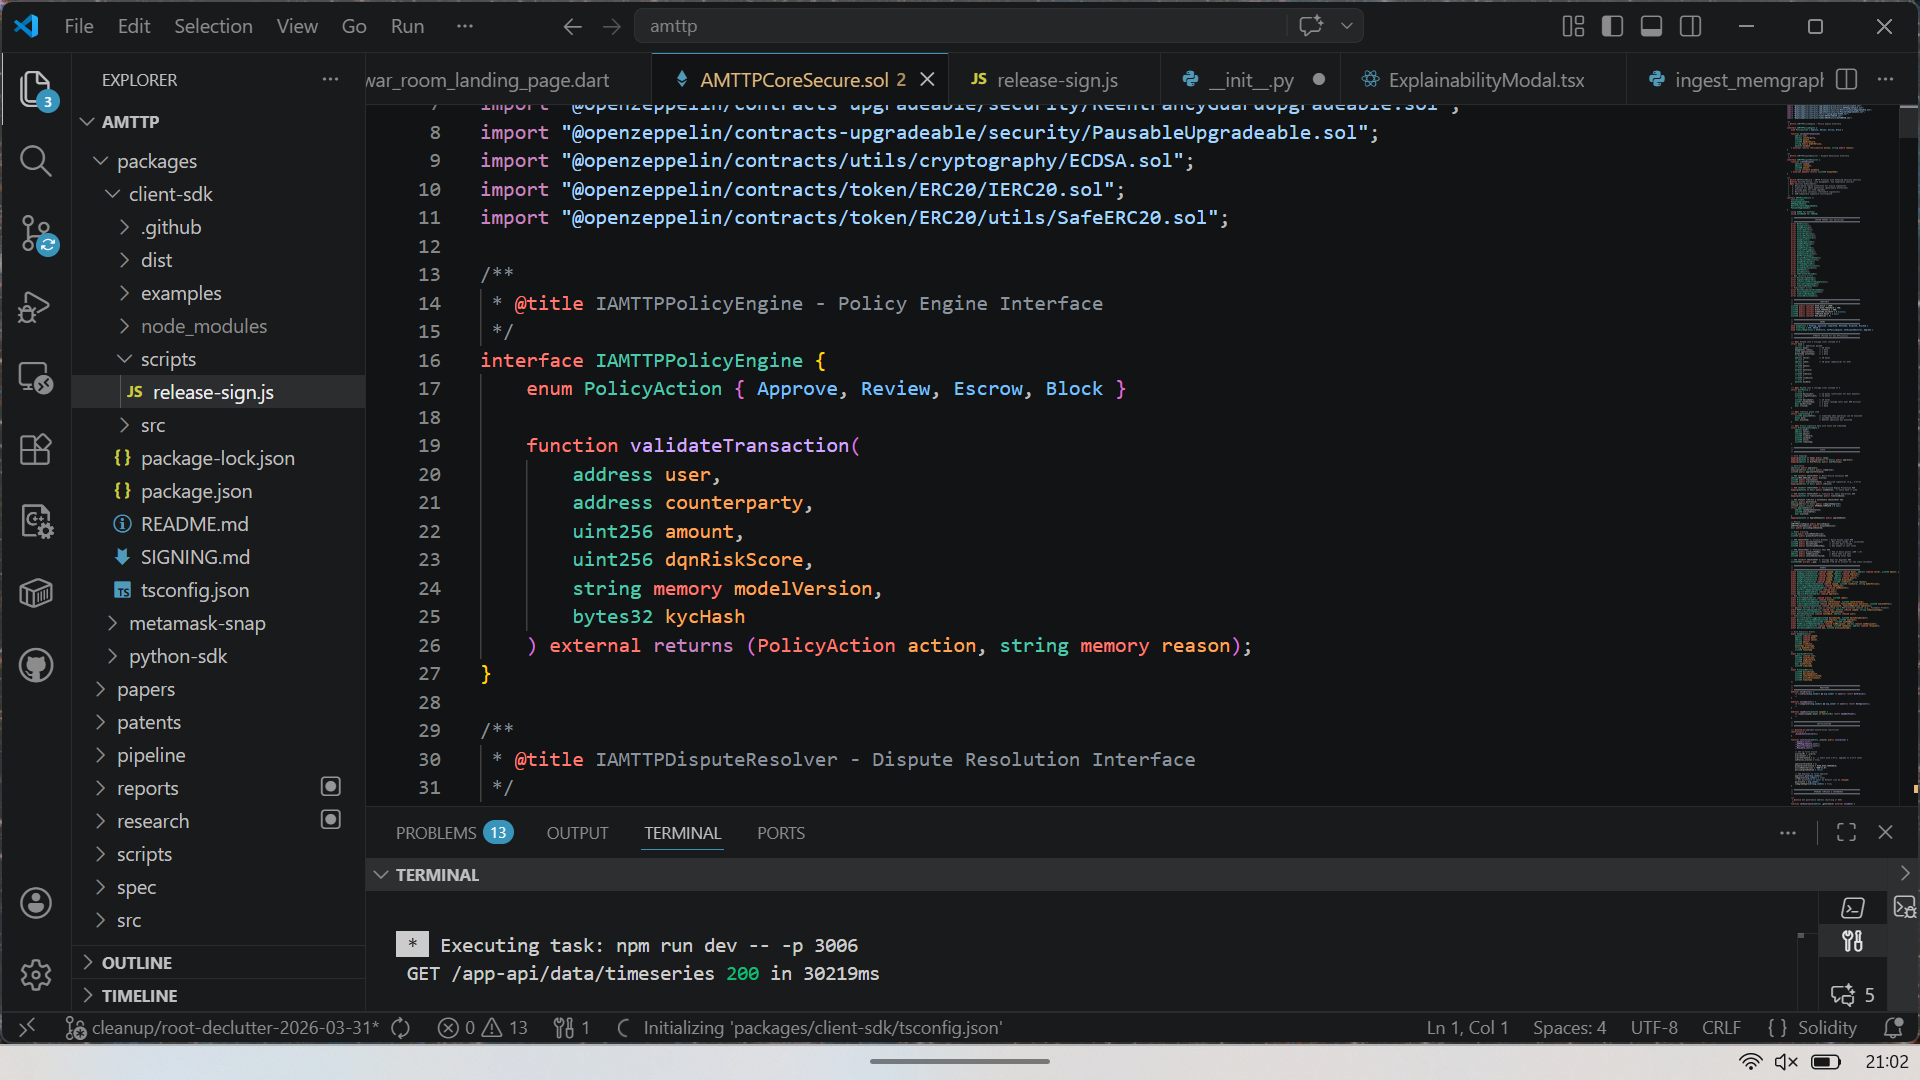
\includegraphics[width=0.97\textwidth]{images/vscode_multitab.png}
\end{center}
\noindent\textit{Figure 1: VS Code showing \texttt{AMTTPCoreSecure.sol} --- the \texttt{IAMTTPPolicyEngine} interface defining the deterministic compliance decision enum (\texttt{Approve, Review, Escrow, Block}) and the \texttt{validateTransaction} function accepting risk score, KYC hash, and model version inputs. The terminal confirms the Next.js War Room dev server (port 3006) running live. Multiple files open simultaneously: Flutter (\texttt{.dart}), Solidity (\texttt{.sol}), JavaScript, Python, and TypeScript --- confirming sole polyglot authorship across all five languages.}

\section*{3. Contract Compilation and Test Results}

\vspace{0.1cm}
\begin{center}
    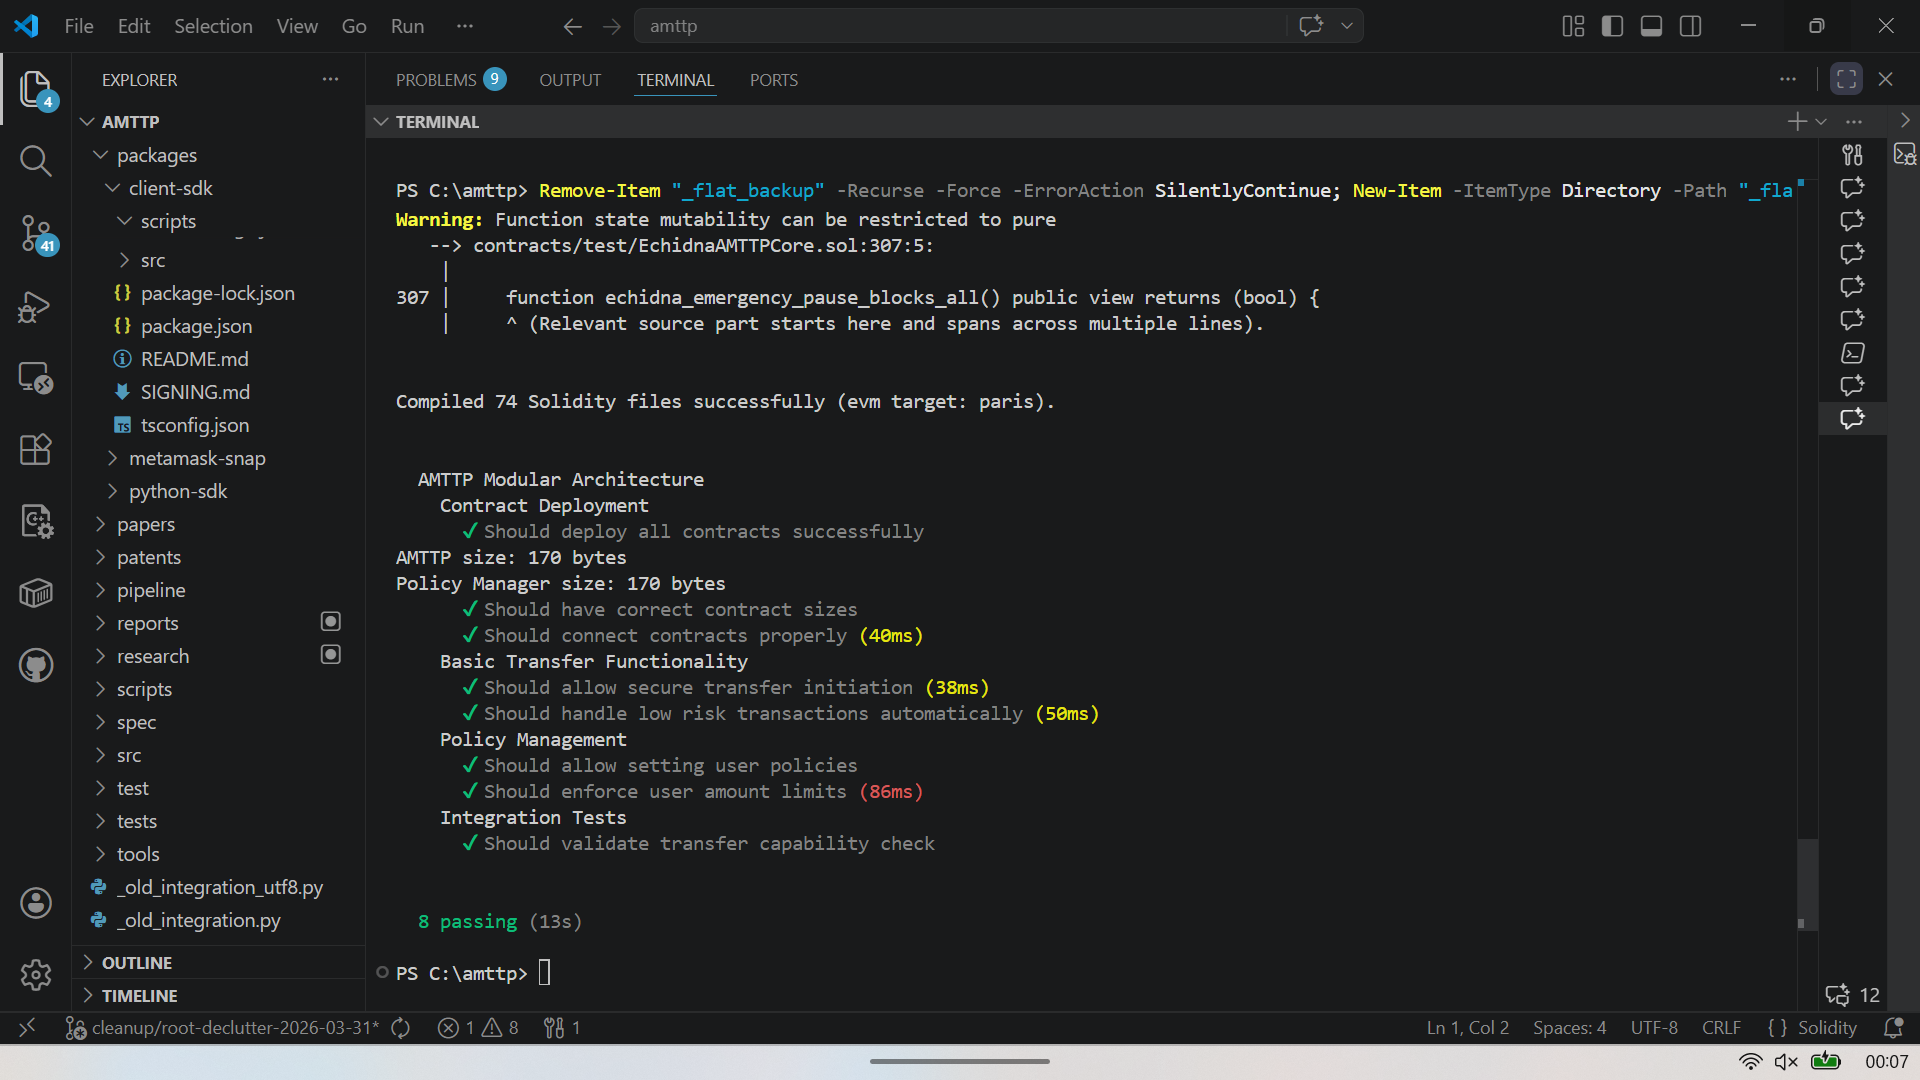
\includegraphics[width=0.97\textwidth]{images/vscode_hardhat_tests.png}
\end{center}
\noindent\textit{Figure 2: Hardhat test output confirming successful compilation of \textbf{74 Solidity files} and \textbf{8 passing integration tests} covering: Contract Deployment, Policy Manager sizing, Basic Transfer Functionality (secure initiation, low-risk auto-approval), Policy Management (user policies, amount limits), and Integration Tests (transfer capability validation). All tests pass in 13 seconds. The left panel shows the full AMTTP monorepo structure including \texttt{contracts/}, \texttt{backend/}, \texttt{pipeline/}, \texttt{research/}, and \texttt{patents/} directories.}

\section*{4. Engineering Significance}

\begin{itemize}
    \item \textbf{74 Solidity files compiled} --- spanning UUPS proxy contracts, ZK-SNARK verifiers, cross-chain bridges, and the core policy engine
    \item \textbf{IAMTTPPolicyEngine interface} --- defines the \texttt{PolicyAction} enum (\texttt{Approve / Review / Escrow / Block}) consumed by the compliance orchestrator, creating a verifiable on-chain enforcement contract
    \item \textbf{Polyglot authorship} --- simultaneous open files in Dart, Solidity, JavaScript, Python, and TypeScript confirm the applicant personally authored all five language layers of the system without external assistance
    \item \textbf{Test-driven development} --- verified contract behaviour through integration tests, not merely compilation, evidencing production-grade engineering practice
\end{itemize}

\noindent Repository: \texttt{github.com/segetii/AMTTP} | Smart contracts: \texttt{contracts/} directory

\end{document}
